\documentclass[11pt]{scrartcl}
\usepackage[parfill]{parskip}
\usepackage{graphicx}
\usepackage{booktabs}
\usepackage{tabulary}
\usepackage{float}
\usepackage{hyperref}

\usepackage{tikz}

\usetikzlibrary{matrix}

\graphicspath{{../images/}}

\title{\textbf{Case Studies II - Community Talks}}
\subtitle{Technologies and Contributions}
\author{Ricardo Garc\'ia Fern\'andez}
\date{\today}

\begin{document}

\maketitle

\vfill

\begin{flushright}
    \copyright  2013 Ricardo Garc\'ia Fern\'andez - ricardogarfe [at] gmail [dot] com.

    This work is licensed under a Creative Commons 3.0 Unported License.
    To view a copy of this license visit:
 
    \url{http://creativecommons.org/licenses/by/3.0/legalcode}.
\end{flushright}

\begin{figure}[h]
    \begin{flushright}	
        
\includegraphics{by}
        \label{fig:by}
    \end{flushright}
\end{figure}

\newpage

\tableofcontents

\newpage

\pagenumbering{arabic}

\section{Introduction}
\label{sec:introduction}

\par Through this document I want to summarize relation between technologies and contributions in those FLOSS project talks from Subject Case Studies II at URJC. A brief introduction to them and a final comparison table.

% section introduction (end)
\section{Apache Software Foundation}
\label{sec:asf}

\textit{Apache Software Foundation} - \textbf{ASF} - \href{http://en.wikipedia.org/wiki/501(c)_organization#501.28c.29.283.29}{501.3 epigraph C nonprofit Foundation}

ASF defines itself as:
\begin{quotation}
    \emph{"not simply a group of projects sharing a server, but rather a community of developers and users"}
\end{quotation}

A \textit{Foundation} is a legal umbrella to allow us to legality providing transparency.

\subsection{Technologies}

\par Apache could be defined as a community of communities. Therefore contributors enter for each community through its rules. The basic rules are inherited and common from ASF.

\par To make a contribution, first, the contributor must be in contact with the particular community and its ecosystem project.pse, EUPL, FLOSS, FLOSSIE, flos

\par In Apache projects bear a similarity in ecosystems, because they have been through an acceptance process to be adopted or published by Apache.

\par As each project has:
\begin{itemize}
	\item \textit{Mailing lists}.
	\item \textit{Source code}.
	\item \textit{Bug tracking}.
	\item \textit{Mentors}.
	\item \textit{Committers}.
	\item \textit{Documentation} (wikis, html, pdf...).
\end{itemize} Therefore, in order to help you to follow the guidelines set. It is recommended in all FLOSS projects you can register for mailing lists as a first step to find out how it works and basic communication. Then begin to understand the design, installation, use and testing.

\par You can read a summary of the basic rules for contributors \url {http://www.apache.org/dev/contributors.html} ASF.

\par To become a contributor, you have to be invited by the other contributors of the project. Having won merits and respect within the community.

\subsection{How to Contribute}

\par If you want to become a contributor in a project at Apache Software Foundation, a tip, you could start following \href{http://incubator.apache.org/}{incubator projects}.

\begin{figure}[htp]
    \centering
    
\includegraphics[width=0.7\textwidth]{egg-logo.png}
    \caption{Apache Incubator}
    \label{egg-logo}
\end{figure}

\par For a project, this is the previous step before become an Apache project. These projects are looking for create a hudge community and it's easier to become a contributor than in bigger projects from ASF.

\par Every new committer must read Apache Software Foundation Guide introducing all aspects that are needed for a committer:

\begin{itemize}
	\item \textit{Contributor License Agreement} - to contribute with your commits to ASF.
	\item \textit{Account creation} - step by step using ASF standards.
	\item \textit{Responsibilities} - as a member of ASF, personal web space, community, ApacheCon.
\end{itemize} You can find an extense explanation in \href{http://www.apache.org/dev/new-committers-guide.html}{ASF new committers guide}.

\subsection{Committers resources}

\par An interesting link of how decisions are made in the Apache Software Foundations to see meritocracy in action:
\begin{itemize}
	\item \url{http://community.apache.org/committers/}
\end{itemize}

% section  (end)
\section{WebKit}
\label{sec:webkit}

\par \emph{WebKit} is a layout engine software designed to allow web browsers to render html (is not only on web pages). Become a FLOSS project in 2005 when Apple released the code.

\par Is used in Mac OS X system framework with Safari, Dashboard, Mail, and many other OS X applications. Also you can find WebKit in Nintendo 3Ds, Kindle and Android.

\par This project started as a branch of the KHTML and KJS libraries from KDE. It is a community made ​​up by companies: Apple, Nokia, Google, RIM, Igalia, Samsung. Because most contributions are made by companies, I want to emphasize that the company that provides more code to WebKit is Google.It is strange to see this information on a project controlled by Apple.

\begin{figure}[H]
    \centering
    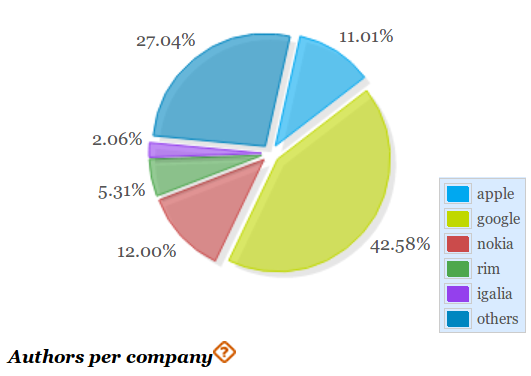
\includegraphics[width=0.7\textwidth]{bitergia-webkit}
    \caption{Bitergia WebKit analysis: \url{http://bitergia.com/public/reports/webkit/2013_01/}}
    \label{}
\end{figure}

\par You can see better numbers in the study by Bitergia on WebKit community posted on February 6, 2013, \href{http://blog.bitergia.com/2013/02/06/report-on-the-activity-of-companies-in-the-webkit-project/}{Bitergia blog}.

\subsection{Technologies}

\par Documentation :The technologies surrounding the WebKit project, which we consider as ALM Tools, (Application Lifecycle Management):

\begin{itemize}
	\item Bug Traking System (BTS) Bugzilla - \url{https://bugs.webkit.org/}
	\item Issue Tracking System (ITS) Trac - \url{http://trac.webkit.org/}
	\item Early Warning Systems (EWS) Bugzilla - \url{http://webkit-commit-queue.appspot.com/}
	\item Developer Guides for each Operative System - \url{http://www.webkit.org/building/tools.html}
\end{itemize}

\par I will highlight as the \textbf{EWS} tool. \textit{EWS} offers a tracking code contribution we have made to the project (via a patch). It reflects the results of each test in each type of platform. WebKit looks much the appearance of the test because a change can affect millions of users.

\par As we can see, the system shows a first image of the \href{http://webkit-commit-queue.appspot.com/}{status of contributions}.

\begin{figure}[htp]
    \centering
    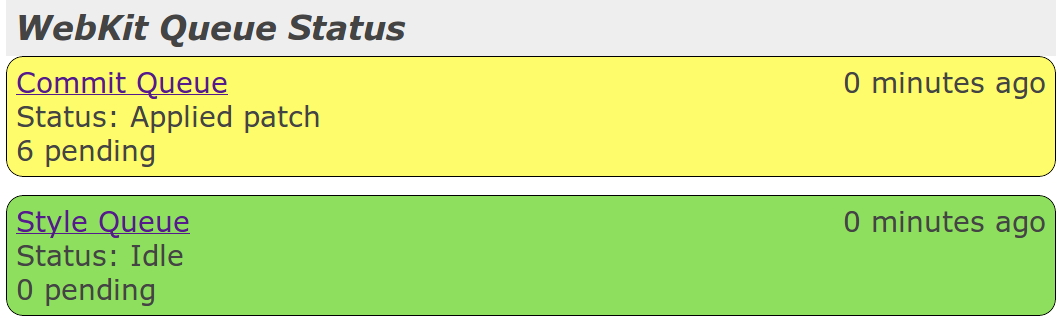
\includegraphics[width=0.7\textwidth]{webkit-queue-status}
    \caption{Queue status}
    \label{queue-status}
\end{figure}

\par Accessing \href{http://build.webkit.org/console}{BuildBot WebKit Console}, we have access to the results and follow-up of each of the patches and tests for each of the existing distributions (ports).

\begin{figure}[htp]
    \centering
    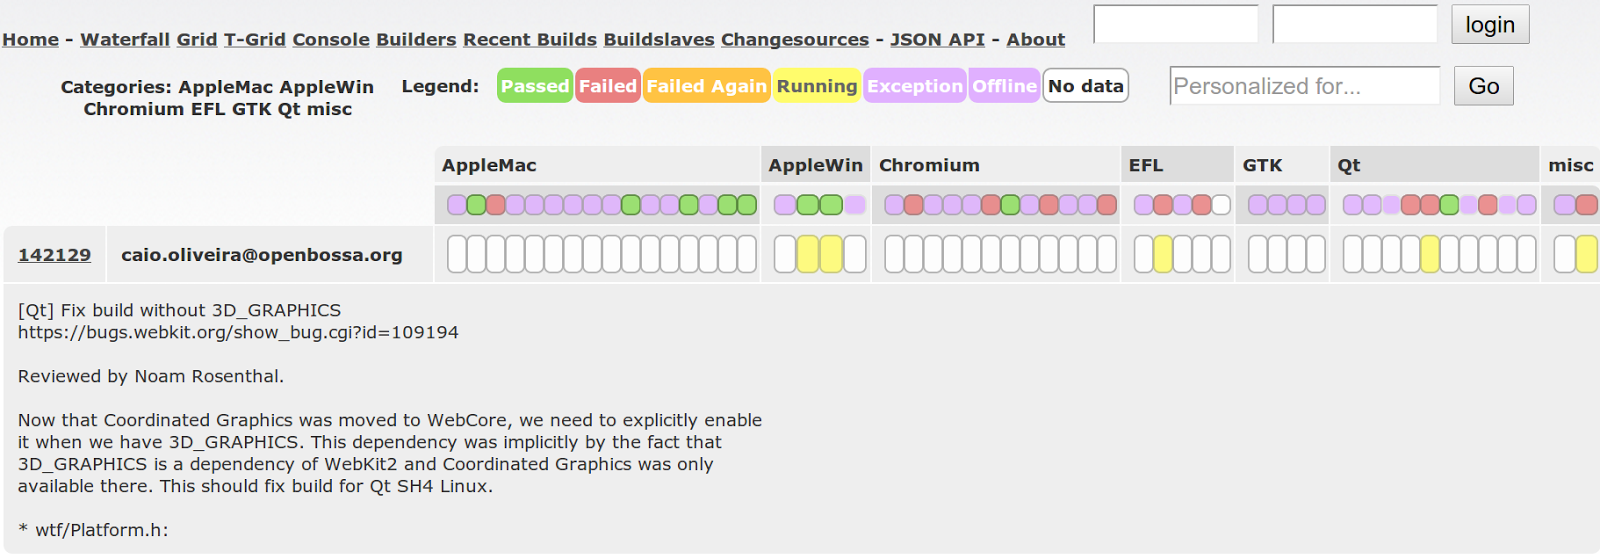
\includegraphics[width=0.7\textwidth]{webkit-build-bot.png}
    \caption{Webkit build bot}
    \label{build-bot}
\end{figure}

\par It is very rigorous system of contributions to the project, we will see in the next section.

\par WebKit has a very useful development guidelines documentation:

\begin{itemize}
	\item \textit{Coding style guidelines} - \url{http://www.webkit.org/coding/coding-style.html}
	\item \textit{Technical Articles} - \url{http://www.webkit.org/coding/technical-articles.html}
	\item \textit{Regression Testing} - \url{http://www.webkit.org/quality/testing.html}
	\item \textit{Reporting Bugs} - \url{http://www.webkit.org/quality/reporting.html}
	\item \textit{Bug Life Cycle} - \url{http://www.webkit.org/quality/lifecycle.html}
	\item \textit{Wiki Documentation} - \url{http://trac.webkit.org/wiki}
\end{itemize}

\subsection{How to Contribute}

\par In WebKit there are many ways of contributions; translations, code, documentation, etc. We are going to focus on contribute with code.
\par There is a guideline explaining \href{http://www.webkit.org/coding/contributing.html}{how to contribute code}. These are the steps you have to follow to contribute code in WebKit:
\begin{itemize}
	\item Choose or create a bug report to work on.
	\item Develop your changes.
	\item Make sure your changes meet the code style guidelines. The check-webkit-style script may be of help.
	\item Run the layout tests using the run-webkit-tests script and make sure they all pass. See the testing page for more information, as well as what you need to do if you've modified JavaScriptCore.
	\item Add any new files to your working directory.
	\item Prepare a change log entry. You may have to add entries to multiple ChangeLogs. The prepare-ChangeLog script will create stub entries for you. See the paragraph about ChangeLogs below.
	\item Create the patch using the svn-create-patch script.
	\item Submit your patch for review to bugs.webkit.org.
	\item Make any changes recommended by the reviewer.
	\item Once reviewed, ask someone to land your patch or mark it for automated commit.
	\item Please watch for any regressions it may have caused (hopefully none)!
\end{itemize}

\subsubsection{Committers and Reviewers}

\par WebKit contributors are divided into two groups; \textit{committers} and \textit{reviewers}. The committers can contribute code to the reviewers agree.

\par \textit{To be a committer}, you have to be nominated by the reviewers. Having a minimum number of significant patches \textit{(ranges between 10 and 20)}. Bureaucratic process and receive approval of 3. Is searching the plurality of contacting between one or more reviewers.

\begin{quotation}
    \textit{Any company with more than three reviewers may give permission to a reviewer.}
\end{quotation}

\par Becoming reviewer, is a higher jump. You have been elected by \textit{reviewers from different companies and have contributed over 80 functional patches}.

\par Both steps are accompanied by the signing of an agreement with Apple, not with the WebKit project.

% section webkit (end)
\section{Plan 9}
\label{sec:plan9}

\par What is Plan9 ? A movie from Ed Wood ? A 'new' Operative System ?\textit{Plan9 from Bell Labs} is an Operative System developed \href{http://swtch.com/plan9history/}{between the 80's and 2002} by the research and development subsidiary of the French-owned Alcatel-Lucent in Berkeley Heights, New Jersey, United States.\textit{Yes, the name is from the movie :)}

\begin{figure}[H]
\centering
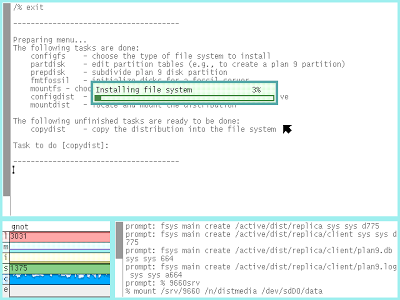
\includegraphics[width=\textwidth]{plan9-install}
\caption{Plan9 talk by \textit{Enrique Soriano Salvador}}
\label{plan9-film}
\end{figure}

\par Plan9 was developed by the same developers of Unix to create a real network OS where \textit{everything} is a file. Even the processes. Everything is related to the basic input/output file readers, the main purpose in the ancient Unix.

\subsection{Technologies}

\textit{Plan9}is developed using C language. The tools they use to collaborate are:
\begin{itemize}
	\item \textit{Mail lists} - to get in touch with the community and contribute tool \url{http://plan9.bell-labs.com/wiki/plan9/mailing_lists}.
	\item \textit{patch} - Command (\href{http://plan9.bell-labs.com/magic/man2html/1/patch}{\textit{patch}})to create file changes.
	\item \textit{Online Sources} -\url{http://plan9.bell-labs.com/sources/}
	\item \textit{TODO} -\url{http://plan9.bell-labs.com/wiki/plan9/TODO/index.html}
	\item \textit{Contrib index} -\url{http://plan9.bell-labs.com/wiki/plan9/Contrib_index/index.html}
	\item \textit{Irc channel} -\url{http://plan9.bell-labs.com/wiki/plan9/IRC/index.html}
	\item \textit{Workshops} - \url{http://www.iwp9.org/}
\end{itemize}

\subsection{How to Contribute}

\par Contributing to the community is difficult, because all your contributions have to pass Plan9 filter handled by one person. You don't depend on a community itself.

\par By other way, you have a very good guidelines and references by very good C developers to \href{http://plan9.bell-labs.com/magic/man2html/6/style}{develop Plan9}.

\begin{itemize}
	\item don't use // comments; some old Plan 9 code does, but we're converting it as we touch it. We do sometimes use // to comment-out a few lines of code.
	\item avoid gotos.
	\item no tabs expanded to spaces.
	\item no white space before opening braces.
	\item no white space after the word "if", "for", "while", etc.
	\item no braces around single-line blocks (e.g., if, for, and while bodies).
	\item integer-valued functions return -1 on error, 0 or positive on success.
	\item functions that return errors should set errstr(2).
	\item variable and function names are all lowercase, with no underscores.
	\item enum or \#defined constants should be Uppercase or UPPERCASE.
	\item struct tags are Uppercase, with matching typedefs.
	\item automatic variables (local variables inside a function) are never initialized at declaration.
	\item follow the standard idioms: use x$<$0 not 0$>$x, etc.
\end{itemize} The end they follow a very common development filosophy:

\begin{quotation}
    \textit{Ultimately, the goal is to write code that fits in with the other code around it and the system as a whole. If the file you are editing already deviates from these guidelines, do what it does. After you edit a file, a reader should not be able to tell just from coding style which parts you worked on.}
\end{quotation}

\par In my opinion, \textit{Plan9 is a very good Operative System to learn how an Operative System works and enjoy learning}.

% section plan9 (end)
\section{Mozilla}
\label{sec:mozilla}

\par \href{http://www.mozilla.org/}{Mozilla foundation} is a huge community that involves different types of users and has a central message applied to all its levels:

\par \textit{"Our mission is to promote openness, innovation \& opportunity on the Web."} In \href{http://www.mozilla.org/about/manifesto.html}{Mozilla Manifesto} you can read the whole document about freedom and accessibility that they apply day by day.

\par The Foundation is consolidated by years of dedication to freedom of the web through its flagship Firefox. Since Netscape released the source code in 1998 Mozilla got down to work to develop a web browser from FLOSS source code they received from Netscape.

\par Mozilla wanted a free internet because IExplorer market share was 90\%. Was a private market and now this trend has changed. Source: \href{http://gs.statcounter.com/#browser-ww-yearly-2008-2013}{StatCounter Global Stats - Browser Market Share}

\subsection{Technologies}

\par There is a bunch of technologies surrounding Mozilla development communities and of course, projects:

\begin{itemize}
	\item \textit{Firefox} - Web Browser with a particularity that doesn't have portability to IOS because it uses Gecko instead of Webkit to render content. Apple doesn't allow a browser (or anything) that is not reder using Webkit.
	\item \textit{FirefoxOS} - New Mobile operative system based in HTML5 and Browser Oriented.
	\item \textit{Thunderbird} - eMail management but abandoned project. Developers have changed to Mozilla.
	\item \textit{Camino} - MacOS Mozilla Browser using Webkit
	\item \textit{Seamonkey} - Firefox, Thunderbird, Chat, Web Editor.
	\item \textit{Sundbird/Lightning} - Calendar project from Mozilla.
	\item \textit{XULRunner} - It's like Java Virtual Machine allowing multiplatform products oriented to Mozilla packages.
\end{itemize}

And of course, developer tools to work with Mozilla community:

\begin{itemize}
	\item \textit{Mailing lists}- For developers, information, everything related to \href{https://lists.mozilla.org/listinfo}{Mozilla}.
	\item \textit{Bug Tracking System}-\href{https://bugzilla.mozilla.org/}{Bugzilla}for every product.
	\item \textit{Source Code Management}- Baazar, Mercurial, SVN, CVS.
	\item \textit{MXR}- Cross references about the code from Mozilla (\href{http://mxr.mozilla.org/}{mxr}).
	\item \textit{Forge for scm}- GitHub.
	\item \textit{QMO}-Home of Mozilla's testing and \href{http://quality.mozilla.org/}{quality assurance community}.
	\item \textit{Crash Stats} - \emph{Continuous integration} server output visualizations using \href{https://github.com/mozilla/socorro}{Socorro}.
	\item \textit{Graph CI}- Graphic visualization for every built from the code in\href{http://graphs.mozilla.org/}{graph section}.
	\item \textit{Tinderbox}- Tool to navigate through \href{http://tinderbox.mozilla.org/showbuilds.cgi}{build logs and results}.
\end{itemize}

\subsection{How to contribute}

\par Mozilla community is very community, this statement may sound redundant, but would be an accurate definition. He moved away from the technology and developers as standard for any project.

\begin{figure}[H]
    \centering
    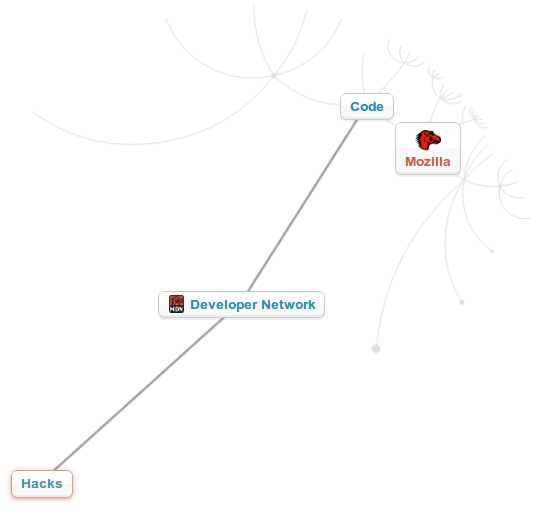
\includegraphics[width=0.7\textwidth]{mozilla-community-developers}
    \caption{}
    \label{community-dev}
\end{figure}

\par Mozilla has the basic steps as other FLOSS projects for \href{http://www.mozilla.org/es-ES/contribute/}{How to Contribute} and gives you an opportunity to contribute in more than one way looking for a chance:

\begin{itemize}
	\item Help for Users
	\item Quality control
	\item Programming
	\item Spread the word
	\item location
	\item Web Development
	\item Accessories
	\item graphic Design
	\item Documentation and drafting
	\item Education
\end{itemize}

\par Furthermore gives you the opportunity to look for contribution near your location, a very useful tool. Mozilla invites you to be part of an Open Web. You don't have to be the smartest guy in the world they do this work spreading that all help is good an they will find for you the best place to help \textit{everyone} with your contribution.

% section mozilla (end)

\section{GNU}
\label{sec:gnu}

Starting with the acronym inception definition of GNU \textit{"GNU is not Unix!"} in 1983. GNU is divided in three departments:
\begin{itemize}
	\item \textit{The GNU Project}.
	\item \textit{GNU Software} - Develops GNU software.
	\item \textit{The GNU System} - GNU Software + external Software.
\end{itemize}

\par GNU selected Unix because of simplicity instead of VMS. Composed by different independent utilities. Decoupled and modular, so the choice to clone the system.

\par \textit{GNU Project} is a Global Project, hasn’t legal entity. RMS (Richard Matthew Stallman) created \textit{Free Software Foundation} (FSF) to convert legal resources to GNU hackers.

\subsection{Techonologies}

\par All projects inside GNU universe share a homogeneous structure and tools to contribute. A part from common techonoligies they use specific tools for each project, depending of the tool purpose.

\par Here is a common list for every GNU project:

\begin{itemize}
	\item Webpage
	\item Development
	\item Manual
	\item Reporting bugs
	\item Getting help
\end{itemize}

\par We apply this structure to an existing GNU project: \href{http://www.gnu.org/software/recutils/}{GNU Recutils}and see how easy is to get all starter information.

\textit{GNU Recutils} is a set of tools and libraries to access human-editable, plain text databases called recfiles.

\begin{itemize}
	\item Webpage -\url{http://www.gnu.org/software/recutils/}{http://www.gnu.org/software/recutils/}
	\item Development -\url{http://savannah.gnu.org/projects/recutils/}{http://savannah.gnu.org/projects/recutils/}
	\item Manual -\url{http://www.gnu.org/software/recutils/manual/}{http://www.gnu.org/software/recutils/manual/}
	\item Reporting bugs -\url{http://savannah.gnu.org/bugs/?group=recutils}{http://savannah.gnu.org/bugs/?group=recutils}
	\item Getting help - FAQ\url{http://www.gnu.org/software/recutils/faq.html}{http://www.gnu.org/software/recutils/faq.html}
	\item Mailing lists - bugs\url{http://lists.gnu.org/mailman/listinfo/bug-recutils} and help\url{http://lists.gnu.org/mailman/listinfo/help-recutils}.
\end{itemize}

\par You have total freedom from the moment when develop, test, and evolve Recutils from tools or guides that offer.

\par At last but not least important: Following \href{http://www.gnu.org/prep/standards/}{GNU coding standards} that are very important to develop readable code.

\subsection{How to Contribute}

\par At this section you will wonder, how I can contribute in a GNU project? one of the most important projects in history?It's easier than it at first seems, of course, following some basic rules of coordination and participation.

\par In an overall picture youcan recognize this structure:

\begin{itemize}
	\item \textit{RMS} - Appoints maintainers. \textit{"GNUism"}.
	\item \textit{GNU Advisory Committe} (2009) - Advisory, communication, transversal vision, external contact. advisory@gnu.org. 8 people, most maintainers and FSF America and Europe vice-presidents.
	\item \textit{Maintainers} - Maintainer, lead program development. Follow \href{http://www.gnu.org/prep/maintain_toc.html}{GNU policies for maintainers}.
	\item \textit{Contributors} - Developers with or without commit access.
\end{itemize} You start in the last point as a contributor with ot without commit access, because GNU is not only writting code. There are many areas: documentation, translations, blogging, law, in which where you can be more helpfull that you think. Take a tour in \href{http://www.gnu.org/help/}{How to help GNU}.

\par But, focussing strictly on development you start as a non commit contributor, inside a mailing list following basic guides. Explaining Recutils project guidelines:

\begin{itemize}
	\item \textit{Test releases} - Trying the latest test release (when available) is always appreciated. Test releases of Recutils can be found at http://alpha.gnu.org/gnu/recutils/ (via HTTP) and ftp://alpha.gnu.org/gnu/recutils/ (via FTP).
	\item \textit{Development} - For development sources, bug and patch trackers, and other information, please see the Recutils project page at savannah.gnu.org.
	\item \textit{Translating Recutils} - To translate Recutils's messages into other languages, please see the Translation Project page for Recutils. If you have a new translation of the message strings, or updates to the existing strings, please have the changes made in this repository. Only translations from this site will be incorporated into Recutils. For more information, see the Translation Project.
	\item \textit{Maintainer} - Recutils is currently being maintained by Jose E. Marchesi. Please use the mailing lists for contact.
\end{itemize}

\par Starting from these test releases to get an inmersion in the project and know its architecture. This starting point is very important for FLOSS project because is an starting mentoring guide through the code and project structure.

\par After this step you can know how to read (better not perfectly) the code, understand bugs, follow solutions and develop your first patch. Here is your gateway to contribute with code to a GNU Project and the path to become a maintainer, only if you want to learn (for 'gratis').

\par Other ways to contribute, as I explained before, are translate projects and develop documentation. Jos\'e E. Marchesithat explains what is and what gives you 'Software Libre': \href{http://es.gnu.org/~jemarch/bicicletas.html}{Bicicletas y Software Libre}.

\begin{quotation}
    \emph{Ayer me compr\'e una bicicleta. ¡Y es algo fant\'astico! Puedo utilizarla tanto en la ciudad como en el campo. ¡Y en cualquier mes del año! Puedo darme paseos y, si alg\'un d\'ia me hace falta, puedo repartir peri\'odicos y sacarme unos durillos. Mi bici no tra\'ia luces, pero no es problema: le he puesto una dinamo y una buena luz, incluso lo he hecho yo mismo: ¡ahorras y aprendes al mismo tiempo! Adem\'as la hemos pagado a medias entre mi compañera y yo. No es ning\'un problema compartirla. Pero quiz\'a alg\'un d\'ia nos cansemos y queramos librarnos de ella. Podremos venderla de segunda mano. O se la regalaremos a alguien que la vaya a usar.
    \\ Hoy me he comprado un programa de ordenador. No es nada muy sofisticado (un cliente para leer el correo), pero tiene buena pinta y hace mogoll\'on de cosas. Me ha salido bastante caro porque no he podido comprarlo a medias. Me dicen que ella no puede utilizarlo, aunque lo necesita. Adem\'as s\'olo podr\'e utilizarlo durante un año. Me han dicho que pasado ese tiempo debo pagarlo otra vez y usarlo durante un año m\'as y no puedo engañarles: el programa se rompe y ya no funciona m\'as. Curiosamente he le\'ido que si utilizo este programa en Corea del Norte ser\'a ilegal. ¡Menos mal que no planeo viajar por all\'i! Esta compra no me va a salir nada rentable porque tampoco debo utilizarlo para ganar dinero. “Uso no comercial”, dicen.
    \\ Luego en casa me he dado cuenta de que el programa usa una letra muy pequeña y no veo bien las cosas. Se lo he llevado a un primo m\'io inform\'atico a ver si me lo pod\'ia arreglar, pero me ha dicho que no puede, que es ilegal. Ya no quiero el programa (estoy muy enfadado) pero no puedo venderlo ni regal\'arselo a nadie: tambi\'en est\'a prohibido.
    \\ Me dice mi primo que esto se llama “modelo de mercado del software privativo” y que lleg\'o a principios de los ‘80. Pero dice que existe una alternativa llamada software libre. “¿Y c\'omo es eso?”, le pregunt\'e. “F\'acil”, contest\'o, “es como comprarte una bicicleta”.}
\end{quotation}

% section gnu (end)
\section{Document Foundation}
\label{sec:document-foundation}

Charles H. Schulz:

\begin{quote}
    \textit{"keeping languages and cultures in this century needs to have fully complete location software"}
\end{quote}

Oracle bought Sun in 2009 (\textit{lots of stories have started here since this date :)}). This affects to \href{http://www.openoffice.org/}{OpenOffice}development before (Sun crisis didn't provide founds to the project), after (New company, new roles, new organization) and then, Oracle semi-abandoned OpenOffice efforts: disappeared references from web pages, guidance and roadmaps. All the work that OpenOffice was doing for 10 years was near todisappear The project will stop to exist and the project members had to prepare and founded \textit{The Document Foundation} and the \textbf{\href{http://www.documentfoundation.org/foundation}{Manifesto}}

\begin{quote}
    \textit{"For the past ten years, the OpenOffice.org community has developed, supported and promoted the world's leading open-source office productivity suite. We have attracted the support of tens of thousands of individuals and corporate bodies during this period. We now call on all our supporters to follow us into the next phase of our development, as we become an independent Foundation."}
\end{quote}

\par Leaded by proposing available FLOSS projects to people. From this date The Document Foundation created LibreOffice to continue development of an FLOSS Office solution to people. This was the born of \textit{LibreOffice}. Now available 4.0version while I'm writing these lines.

\subsection{Technologies}

\par The basic rule in a FLOSS project is \textit{"show me the code"}. Thus as is in LibreOffice, get into the code and communication channels to create an easy development tools forge.

\begin{itemize}
	\item \textit{Distributed repository} - Chose git as social and cultural decision instead of other options like Mercurial or Bazaar.\url{http://cgit.freedesktop.org/libreoffice}
	\item \textit{Integration and Revision} - \href{https://gerrit.libreoffice.org/}{Gerrit} project for patches integration (not feature branch).
	\item \textit{Issues Tracking System} - Bugzilla: Social and Cultural decision - \url{https://bugs.freedesktop.org/}
	\item \textit{Wiki} - For contributors, developers, translations, desing in \url{https://wiki.documentfoundation.org/Development}
	\item \textit{Release often Release Earlier} - Fixed release dates - 1 year and half - Have a \textit{\href{https://wiki.documentfoundation.org/ReleasePlan}{Public Roadmap}}. Release often and you will find bugs, and this is good because maintain developers interest.
	\item \textit{License} - LGPL 3.0 and MPL allow downstream from Apache License.
	\item \textit{Mailing Lists}: \href{http://lists.freedesktop.org/mailman/listinfo/libreoffice}{Developers}, questions and answers, etc.
	\item \textit{IRC Channel}:\href{irc://chat.freenode.net/libreoffice-dev}{\#libreoffice-dev channel}to contact developers, users, immediatly.
	\item \textit{Forums}: This channel is the most used and active by developers and users even than the mailing lists -\url{http://es.libreofficeforum.org/}.
\end{itemize} There is a reference guide for first steps with LibreOffice development available at \url{http://www.documentfoundation.org/develop/} with all detailed references.

\subsection{How to Contribute}

\par Charles aimed us to contribute without fear to the project, trying and sending our developments (bugs, features, etc) to mailing list. He saids that all work is well received and more important the code you contribute to the project belongs to you, there are no developer agreement neither ownership transferences in LibreOffice project. \textit{"No Pyramids, self interest"}.

\par To main sections where explained:

\begin{itemize}
	\item \textit{Easy hacks} -\url{https://wiki.documentfoundation.org/Development/Easy_Hacks}. \textit{'Easy' bugs are waiting for you} in this buglist. The first door to contribute and get feedback to get in touch with this big community. These bugs are prepared for people to contribute to the project as a start up page and familiar with community process. I think is a good idea.
	\item \textit{Crazy ideas} - \url{https://wiki.documentfoundation.org/Development/Crazy_Ideas}. The title explains a lot related to this idea, and I like it:\textit{"With a product like LibreOffice, there is often a floodgate of radical ideas on directions the project might take"}. Its a queue to propose new ideas from brainstorming community process, they invite you to contribute in this section will your thoughts, not all will be discussed but where most ideas come together and mixed the best ideas should appear.
\end{itemize}

\par There is a Wiki explaining the process to get involved as LibreOffice contributor: \url{https://wiki.documentfoundation.org/Development#How_to_get_involved}.

\par As in other FLOSS projects \textit{LibreOffice} has a basic guides to contribute in development process and decision making inside the community and how to decisions are made and which way the process become more open, simple and participatory.

\begin{itemize}
	\item \textit{Meritocracy} to propose and defend technological aspects but always has to be argued, always.
	\item \textit{Vote for specific things} - Voting is used lesser but for some decisions is easier to vote, release dates, conferences, workshops, etc.
	\item \textit{Do, don't talk} - Do-cracy, sometimes is better to do that wait or argue to introduce new features, bugs, etc. Distributed Control Systems helps to generate easily new solutions to share with community.
\end{itemize}

\par Process patterns:

\begin{itemize}
	\item \textit{Simple Tools} - As easy as only focus on your goal.
	\item \textit{Simple contribution process} - You came with your patch and present it to the community. No Agreements to give code owner rights, belongs to you.
	\item \textit{Loose structure (teams) }- I could say scalable teams, with a good workflow team are mutable and easy to working with.
	\item \textit{Native language} - Teams duplicate whatever they feel is useful for their project. Free to replicate for every language by each team.
	\item \textit{Transparency} - The most important aspect, transparency, to show the work and be truthful to everyone.
\end{itemize}I suggest you to visit \href{http://standardsandfreedom.net/}{Charles} website and \href{https://wiki.documentfoundation.org/Development#Finding_a_first_task:_Easy_Hacks}{Easy Hacks} section.

% section document-foundation (end)
\section{Libre Desktop}
\label{sec:libre-desktop}
 
\par This is a different talk from others saw in the blog. \textit{Libre Desktops and Public Administrations} talk tries to measure FLOSS \textit{(Free Libre Open Source Software)} Desktop environments success in Spain Public Administration.

\par Main goals of mixing FLOSS software in projects could be resume in:

\begin{itemize}
	\item Balance costs
	\item Reinvest in \textit{"Comunidades Autónomas"}(CCAA).
	\item Develop own solutions.
\end{itemize} Encouraging FLOSS use in Public Administrations becomes a double success for projects and CCAA. 

\par Yes because FLOSS has to be encouraged and must use in every Public project for each country, because is paid with people's money.

\par But is not easy as it seems, because we have the responsability to spread the benefits of using FLOSS licenses, projects, documentation and help possitively to adopt these kind of advantages.
\\ FLOSS doesn't mean GRATIS. I recommend you take a look this \href{http://mastersfwlurjc.blogspot.com.es/2012/11/errores-de-percepcion-del-software-libre.html}{disambiguation in FLOSS} projects that I made before.

\subsection{Transparency}

\par Transparency is a very important word inside FLOSS world and has to be as important in Public Administrations world. All public data belongs to everyone in the country, so starting from this assertion we see the needs of FLOSS licenses in Public Administrations to continue evolving with solutions, adapting our needs and learning from others development. It's the wheel of knowledge, allways hungry.

\subsection{Ministerio de Administraciones Públicas}

\par Miguel Angel Amutio Chief of Planning and Operations area at \textit{Ministerio de Administraciones Públicas}made a study to introduce FLOSS advantages inside CCAA project development in 2005. This translation from FLOSS to human-readable content is necesary to spread FLOSS advantages inside a new area.

\par Main topics could be summarized in:

\begin{itemize}
	\item Overall review of what is FLOSS to define, explain and put into operation in public administration.
	\item Representation of Software as a Service.
	\item Give a chance to negotiate from FLOSS away from slavery to proprietary software.
	\item Investment protection against a Single vendor that can disappear.
	\item Interoperability.
\end{itemize} They aren't weird and extrange for a Software Developer but, for common people (not Pulp's song, the others :))away from the FLOSS world, is not so simple to know these benefits or advantages that it provides. Yes, it provide us, I speak as a citizen which my (our) taxes are invested in IT solutionsdevelopment for public administration.

\par \textit{"Liability management software from FLOSS"}

\par You can see the whole article in \href{http://administracionelectronica.gob.es/?_nfpb=true&amp;_pageLabel=P803324061272301226576&amp;langPae=es&amp;detalleLista=PAE_000001307}{Administraci\'on Electr\'onica website}.

\par This was a very huge step for introduction to FLOSS in Public Administrations in Spain. During those years invest in FLOSS projects grown producing, better solutions, Linux distributions, and training,devoting more resources to the knowledge than the payment of licenses, ie encouraging Public Administrations knowledge.

\subsection{Cenatic \& Libresoft}

\par In 2008 \href{http://www.cenatic.es/sobre-cenatic}{Cenatic} and \href{http://libresoft.es/about}{Libresoft} made an analysis to measure FLOSS implantation success in Public Adminstrations to retrieve more data directly from software developers, not only 'static' data from code.

\begin{itemize}
	\item Quantitative analysis of the public administration.
	\item Based on the experience of government employees (interviews).
\end{itemize}

\href{http://observatorio.cenatic.es/index.php?option=com_content&amp;view=article&amp;id=39:software-de-fuentes-abiertas-para-el-desarrollo-de-la-administracion-publica-espanola-una-vision-global-2008&amp;catid=5:administraciones-publicas&amp;Itemid=21}{Here is} the complete document.

\par After all data retrievement IMHO \textit{(In My Humble Opinion)}, the most important thing is to spread the virtues of using FLOSS in public administrations because this advantage is like a boomerang, closes the circle of knowledge,returning knowledge to people who invest in the creation and use of a public service.

\par Must be able to explain the virtues that gives us the use of FLOSS in any field on the basis that knowledge is free.

% section libre-desktop (end)
\section{Wikipedia}
\label{sec:wikipedia}

I'm not going to introduce what is \href{http://www.wikipedia.org/}{Wikipedia}, you know what Wikipedia is. I will write about what is not and how Wikipedia community is governed by rules using tools for this mean.

\par Everything revolves around \textit{"citation needed"}quotation.
\\\href{http://gsyc.urjc.es/~mvidal/}{Miguel Vidal} explains the Wikipedia community during the talk through the vision of a Wikipedian. A quick look at what is not Wikipedia

\begin{itemize}
	\item Is not a dictionary.
	\item Is not a blog.
	\item Is not a centralized image bucket.
	\item Is not a web of links.
	\item Is not a collection of meaningless information.
\end{itemize} Wikipedia is a Free Encyclopedia \textit{(yes,I failed, I finally described the meaning of wikipedia :))}with \href{http://creativecommons.org/licenses/by-sa/3.0/}{Creative Commons By Share Alike} (CC-BY-SA) License.

\subsection{Technologies}

\par Wikipedia, Wikipedia, Wikis everywhere ! What was before ? Wiki or Wikipedia ? Wiki was created in march of 1995 by\href{http://c2.com/~ward/}{Ward Cunningham} expert software developer, pattern designer and extreme programing pionner. He defined Wiki as \textit{"The simplest online database that could possibly work"}.

\par Wiki is a content management system focused in team collaboration development. Easy collaboration and visualization for a wiki gives disseminated widely results among developers. The key point is the change history associated with each of the pages. The tool allows you to navigate through the story and find out who did what and when. The more information is saved, the more will learn. Then in 2001 he received a big boost from wikipedia to be chosen as the basis for creating the free encyclopedia that during the 2000s was on everyone's lips (anyone who knew the wikipedia), developers, architects, lawyers, children, teachers, etc..

\par The use of wikis is widespread in software development projects as it allows the integration of collaborative document usage. It uses a simple markup language to represent the text in an agile as a html.

\par The Wiki used in Wikipedia is \textit{\href{http://www.mediawiki.org/wiki/MediaWiki}{MediaWiki}} licensed under the \href{http://www.gnu.org/licenses/gpl.html}{GNU GPLv3}. It was developed specifically for the project by \href{http://magnusmanske.de/}{Magnus Manske}. Today has many users who create their Wikis with MediaWiki software.

\par Although the only lack of wikis, is \textit{markup languages​​ unification} and therefore the need for \textit{WYSIWYG} (\textbf{w}hat \textbf{y}ou \textbf{s}ee \textbf{i}s \textbf{w}hat \textbf{y}ou \textbf{g}et) editors for each type of language. At the end, allows to choose one that best suits for each needs.

\subsection{How to Contribute}

\par In Wikipedia contribute is easier that it seems. Go to a Wiki ie \href{http://en.wikipedia.org/wiki/Software_release_life_cycle}{Software release life cycle} and click \textit{edit} button, add your content and save. That's all, no registrations, no forms, no personal data, edit and save.

\begin{figure}[H]
    \centering
    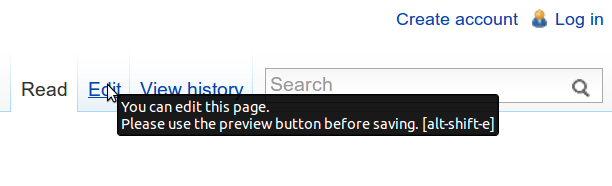
\includegraphics[width=\textwidth]{wiki-edit-button}
    \caption{Wikipedia edit button}
    \label{wiki-edit}
\end{figure}

\par This is your first\textit{affaire}with Wikipedia could be the last only if you want.

Wikipedia has a dedicated domain to Community in \href{http://en.wikipedia.org/wiki/Wikipedia:Community_portal}{Community Portal}:
\begin{quote}
    \textit{"The Community portal is a place to find collaborations, tasks, and news about English Wikipedia."}
\end{quote}

\par There is a guide to start to contribute to Wikipedia throught different ways.

\par \textbf{Important:}Wikipedia is divided in sub communities per each language, this sample is from English Wikipedia.

\begin{itemize}
	\item \textit{Help desk} guides users to learn how to edit using Wiki syntax. How to create an article, describe references, links, citations, relate articles, how to write a Wiki.
	\item In \textit{Reference desk}; you can ask questions to librarians to guide you through Wikipedia inside articles.
	\item \textit{Peer editing} help is a menthoring program for newbies in Wikipedia called TeaHouse. Very interesting part in Community to guide users not only with described rules in more Wikis, community users help to others to interact and use Wikipedia hand by hand with a menthor from Wikipedia. Human communication at least. Very important and appreciated.
	\item \textit{Village pump} is a discussion forum for Wikipedia technical issues, policies, proposals, new ideas. Community discuss policies for Wikipedia reasoning to increase Freedoms in Free Encyclopedia Open Community.
	\item \textit{Dispute resolution}, always are disputes, complains, differences between contributors. This guide tries to resolve them before they exists explaining rules of respect inside Wikipedia and in case you get in the middle of a flame discussion how you can handle this problem and try not to become personal. Always guide yourself from your reasonings.
\end{itemize} I hope you enjoyed and discovered new sections in Wikipedia because is not just an Encyclopedia (Free Encyclopedia :)), is a big community helping each other sharing knowledge with everyone. \textit{People helping people.}

% section wikipedia (end)
\section{Liferay}
\label{sec:liferay}

We can read in liferay.com:
\begin{quote}
    \textit{"Liferay Portal is an enterprise web platform for building business solutions that deliver immediate results and long-term value."}
\end{quote}

\par Translated to human language Liferay is a FLOSS Portal Management System that tends to Content Management System. Nowadays CMS and PMS definitions are converging.

\par Liferay is oriented to Enterprise Portal Managemet. Its main costumer target are companies that purchase \textbf{Enterprise} product and \textbf{Partner} solutions.

\par Liferay encourages community to generate upstream and communications inside the project.

\subsection{Technologies}

\par Liferay is developed in Java and uses \href{http://sourceforge.net/projects/lportal/files/Liferay\%20IDE/1.4.0/liferay-ide-eclipse-updatesite-1.4.0.zip/download}{Eclipse Liferay IDE for developers}. Also needs Liferay Portals and SDK to start developing. With this complete pack you can start developing your own portlets, themes and extensions for Liferay.

\par There is a guide to develop \href{http://www.liferay.com/community/wiki/-/wiki/Main/Liferay+6.0+Development+on+Ubuntu+Maverick+10.10}{Liferay in Ubuntu}explaining from installation to deployment process.

\par Liferay uses Git and has GitHub profile -\url{https://github.com/liferay}. They use GitHub as code reviewer tool linked with JIRA issues and Forum questions.
\par Here is the picture:
\begin{itemize}
	\item Read Documentation guidelines.
	\item Install Liferay Development Environment.
	\item Search for an Issue.
	\item Develop a solution using guidelines.
	\item Make a \textit{pull request} from GitHub to review code.
\end{itemize}

\par Technologies used in contribution process are: \textit{Java, Eclipse, Git, GitHub, Forum and JIRA}. I encourage you to take a tour in next (work in progress) Liferay Development, \textit{\href{http://www.liferay.com/es/documentation/liferay-portal/6.1/user-guide/-/ai/osgi}{OSGI Migration Documentation}.}

\subsection{How to Contribute}

\par Starting from Dashboard first thing you find is a map of global contributions:

\begin{figure}[H]
    \centering
    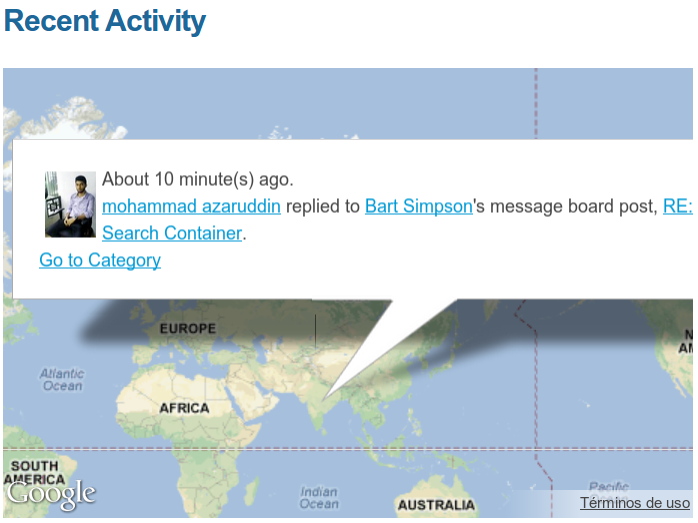
\includegraphics[width=0.7\textwidth]{liferay-dashboard}
    \caption{Liferay Contributions Dashboard}
    \label{dashboard}
\end{figure}

\par Our firs impresion is that Liferay community is developed worldwide. They publish community analysis, workshops, releases and community success samples.

\par It's important to start reading\href{http://www.liferay.com/documentation/liferay-portal/6.1/user-guide}{Liferay user guide}, everyone should start from here, because you need to know first what Liferay is.

\par Liferay encourages users to create a profile page, as we can se \href{http://www.liferay.com/web/jorge.ferrer/profile}{Jorge Ferrer Liferay} personal page. Gives importance to create a 'centralized' community.

\par Like other FLOSS projects they divide community section in two main groups:

\begin{itemize}
	\item Participate -\href{http://www.liferay.com/community/welcome/participate}{http://www.liferay.com/community/welcome/participate}
	\item Contribute -\href{http://www.liferay.com/community/welcome/contribute}{http://www.liferay.com/community/welcome/contribute}
\end{itemize}

\par \textit{Participate} section invites the user to share the experience of liferay, doubts, achievements, proposals, errors found, so that people who encounter the same mistakes do not recur. Thus, creating a place to clarify questions and share knowledge, Liferay community.

\par You can find different ways to communicate with Liferay community, \textit{communicate is as valuable as contribute with code}:

\begin{itemize}
	\item Community Forum
	\item Blogs
	\item Wiki
	\item IRC
	\item Liferay LIVE
	\item Events
	\item Issues
	\item User Groups
\end{itemize}

\par In \textit{Contribute} section you have more technical information about how to contribute 'explicit' with community. \href{http://www.liferay.com/community/wiki/-/wiki/Main/Contributing}{Wiki section} explains different ways and each guide defined to contribute. There is a wide fork to contribute, from translations to writing a complete Liferay plugin:

\begin{itemize}
	\item \textit{Reporting and/or fixing a bug}: \href{http://issues.liferay.com/secure/Dashboard.jspa}{JIRA ITS} is used to provide easy bug/issueTS interface for users. Explained detailed how to report a bug, publish it, search for it and develop a solution.
	\item \href{http://www.liferay.com/community/wiki/-/wiki/Main/Contributing#section-Contributing-Write+documentation}{\textit{Writing documentation}}: In Wiki section is described that every user can write Liferay documentaiton. There are two main guides \textit{Wiki Guidelines} and\textit{Liferay Editorial Guidelines}to contribute with documentation.
	\item \textit{Implementing a new feature}: Section \href{http://www.liferay.com/community/wiki/-/wiki/Proposals/FrontPage}{Proposed Projects} to describe your solution after read and develop your new feature described in \href{http://www.liferay.com/community/wiki/-/wiki/Main/Liferay+Core+Development+Guidelines}{trunk Development Guidelines}. Also you can suggest a new feature in \href{http://www.liferay.com/web/guest/community/forums/-/message_boards/category/1108052}{Liferay Forum}.
	\item \textit{Providing Translations}: Liferay \href{http://www.liferay.com/community/wiki/-/wiki/Main/Translation+Team}{Translation Team}has its own guidelines to manage translation teams for each Language.
	\item \textit{Writing a useful plugin}: They provide a complete developers guide for Liferay plugins in pdf. You can download it \href{http://docs.liferay.com/portal/6.0/official/liferay-developer-guide-6.0.pdf}{here}.
\end{itemize} Ohter remarcable section is \href{http://www.liferay.com/community/ideas}{Community Feature Ideas}. The user can provide ideas to Liferay evolution. Manages JIRA to advertise for Liferay different ideas,JIRA becomes more social and guided by the votes of the people to develop new ideas.

% section liferay (end)
\section{FLOSS Migration}
\label{sec:floss-migration}

\par How is possible a FLOSS migration in Public Administrations ? Here we have \textit{Zaragoza succes case}.

\par \textbf{\href{http://www.zaragoza.es/ciudad/sectores/tecnologia/swlibre/proyecto.htm}{ZO2-AZLINUX}:}FLOSS migration project designed and developed from 2005 in Zaragoza. Inside description we found their slogan:

\begin{quote}
    \textit{"Migration from proprietary software to free software on the computers of municipal employees."}
\end{quote}

\par Migrate private software to FLOSS in Zaragoza Public Administration gradually emphasizing the migration office tools \textit{Microsoft Office} for \textit{OpenOffice} and \textit{Microsoft Windows} operating system for.

\par They developed a migration plan including all actors: politics, technical and users. The whole path to achieve this goal, that all administration could work using FLOSS solutions. Thus Public Administration developments and maintainability is not locked to any private software provided and could invest in Research and Development.

\par This plan is included within a larger plan. Which Zaragoza tries to turn one of the major European cities with greater economic development based on new information technologies and knowledge management.

\par Zaragoza city of knowledge:

\par \url{http://www.zaragoza.es/ciudad/conocimiento/conocimiento.htm}

\subsection{Technologies}

\par Technologies involved to provide same functionality that private software solutions:

\begin{itemize}
	\item 2005 - 2007: Browser Firefox, Thunderbird, Multimedia. Changes soft for positive acceptance.
	\item 2008 - 2010: Office Suites, OpenOffice. Change is harder but accepted.
	\item 2009 - \textasciitilde SO: Switching to OS \href{http://zaragozaciudad.net/azlinux/}{AZLinux}.
\end{itemize} These steps \textbf{must be accompanied} by a parallel track:
\begin{itemize}
	\item \textit{Inventory}: Hardware and Software.
	\item \textit{Communication}: Managing change. Accompany the users through the traumatic process. Talks, cd testing, information exchange process, benefits of using FLOSS
	\item \textit{Technical Training}: An important point to consider.
	\item \textit{Users Training}: 8 hours Windows xp to Linux - 20 hours Office to OpenOffice. \textit{Remarkable time dedicated to users training related to Office Suites higher than OS change}.
\end{itemize}

\subsection{How to Contribute}

\par How could you contribute to this process ? I think the best way to start contributing is to spread this work and its success case to people reluctant to switch to FLOSS. This way is that we have to follow, thus the main reason is the freedom to choose that FLOSS gives you as a user and of course the ability to spread and share knowledge to everyone.

\par After those principles, I want to highlight these links:

\begin{itemize}
	\item Activities -\href{http://www.zaragoza.es/ciudad/sectores/tecnologia/swlibre/actividades_swlibre.htm}{http://www.zaragoza.es/ciudad/sectores/tecnologia/swlibre/actividades\_swlibre.htm}
	\item Open data initiative -\href{http://www.zaragoza.es/ciudad/risp/}{http://www.zaragoza.es/ciudad/risp/}
	\item Promote your applications with open-data -\href{https://www.zaragoza.es/ciudad/enlinea/consulta_risp.xhtm}{https://www.zaragoza.es/ciudad/enlinea/consulta\_risp.xhtm}
\end{itemize}\textit{\textbf{"Open data and FLOSS to serve the people"}}

% section floss-migration (end)
\section{GNOME}
\label{sec:gnome}

\par \textbf{GNOME} is an acronym that means: \textit{GNU Object Model Environment}. Was created in 1997 through the visible momentum of \textit{\href{http://tirania.org/blog/}{Miguel de Icaza}} to provide graphical desktop environments completely FLOSS Linux version build using components and focused on interoperability. Counteract the existing KDE fed on QT (at that time \textbf{was proprietary software, not now}). After some analysis they start developing GNOME using GTK (\textit{\href{http://www.gimp.org/}{Gimp Toolkit}, yes Gimp GNU Image Manipulation Program}:)).

\par \textit{GNOME Foundation} was founded on 15 August 2000 by Compaq, Eazel, Helix Code, IBM, Red Hat and Sun Microsystems. Manages GNOME development and represents GNOME worldwide.

\subsection{Technologies}

\par GNOME is developed using C language and Object Oriented GTK+ library. Each project/module is governed by these basic development tools:

\begin{itemize}
	\item \textit{Maintainer} - benevolent dictator for life for each module. GNOME has a distributed development management divided in modules.
	\item \textit{Mailing list} - Encourage users to develop discussions in mailing list instead of IRC because it is easier to manage the history of the decisions made. \href{https://mail.gnome.org/mailman/listinfo}{Mailing Lists}.
	\item \textit{Bug Tracking System} - \href{https://bugzilla.gnome.org/}{GNOME Bugzilla} manages Project development, Bugs and discussions.
	\item \textit{Documentation} - Wiki is a very useful tool in project development because brings information from the project and its easier to use as a collaborative document development for technical and non-technical users. GNOME Wiki is published in \url{https://live.gnome.org/}.
	\item \textit{Repository} - Distributed repository git in \url{https://git.gnome.org/browse/} and a user guide that explains the use of the repository in live \href{https://live.gnome.org/Git}{Wiki}.
	\item \textit{Synchronous communication} - IRC channel to retrieve information and ask questions related to GNOME. You can find more information in \href{https://live.gnome.org/GnomeIrcChannels}{Wiki} IRC section.
	\item \textit{Quality and Assurance} - Users, the users are the best QA team for Gnome.
\end{itemize} There is a manual for developers specifically dedicated to them, \href{https://developer.gnome.org/}{GNOME Developer Center}. In showing a series of tutorials, documentation and GNOME structure to facilitate the use and implementation of the platform.

\begin{figure}[H]
    \centering
    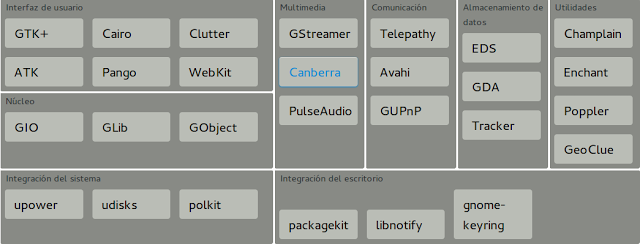
\includegraphics[width=0.7\textwidth]{gnome-system-modules}
    \caption{Gnome platform overview}
    \label{platform}
\end{figure}

\subsection{How to Contribute}

\par GNOME Community has a low barrier entrance guided by Meritocracy. Community guides are available to everyone in \href{https://live.gnome.org/GnomeLove}{GnomeLove}. Here we are going to describe internal process of a contribution and how a contributor reaches the goal of becoming a commiter througth different organization ROLES:

\begin{itemize}
	\item Reasonable number of patches in a module.
	\item Ask for commit rights to Accounts Team
	\item Accounts Team contact module maintainer or translator coordinator to check for approval.
	\item A committer can commit to git repository but her contributions have to be reviewed and approved by maintainer of the module
	\item \textbf{Important}: committers have write access to all git repositories hosted in git.gnome.org. You can contribute to all modules. If you find an error you could fix and commit the patch.
\end{itemize}

\par \textit{Maintainers} are responsible for the module. They have to \textit{review patches} and \textit{assume results}, their role is important inside the community have high responsability. Communications and module releases management are managed by maintainers. Could be various maintainers for one module.

\par Instead of development committers, translators committers in translation modules also are maintainers for themselves because \textit{a translation can't be reviewed} because \textit{it would duplicate the work}. So you have full confidence in the translation module.

% section gnome (end)
\section{Thunderbird Q\&A}
\label{sec:thunderbird-qa}

\par \href{http://www.mozilla.org/es-ES/thunderbird/}{Thunderbird} is a FLOSS Email client from Mozilla Foundation \textit{- MOFO -} . Latest news aren't good news because Mozilla stop development resources to this project on July 2012\footnote{Thunderbird finale - \url{https://blog.lizardwrangler.com/2012/07/06/thunderbird-stability-and-community-innovation/}} but this talk showed us the way developers work in Thunderbird and how Quality \& Assurance \textit{- Q\&A -} Team and developers join efforts to lead a better development.

\par Ludovic Hirliman\footnote{Ludovic Hirliman web - \url{http://perso.hirlimann.net/~ludo/}} is\textit{Q\&A}leader in Thunderbird, through his vision we are capable of see the big picture behind good software development starting with Test Driven Development \textit{- TDD -} .

\begin{center}
    \textit{"Testing Tools: your hand, your brain and time" by Ludovic Hirliman.}
\end{center}

\subsection{Development Tools} "Someone wants to test ? go to url, test and report bugs"Focusing in our goals, here are Thunderbird development tools:
\begin{itemize}
	\item \textit{Bug Tracking Sustem} - Bugzilla - Everyone could post a bug and how to replicate a bug there.
	\item \textit{Test case management software} - \href{https://mail.mozilla.org/pipermail/thunderbird-testers/2012-October/000111.html}{From Litmus to Moztrap}. Tools to create and run test cases related to email clients.
\begin{itemize}
	\item \href{http://litmus.com/}{Limus} - Test interactively with real email clients.
	\item \href{http://moztrap.wordpress.com/}{Moztrap} - Test Case Management from Mozilla.
\end{itemize}
	\item \textit{Continuous Integration} - \href{http://trac.buildbot.net/}{Buildbot} - Checkout, run make, run make test, read log file and automate a build in every commit. Running unit test to build after each commit.
	\item \textit{Documentation} - Wiki to develop extensions and a real user Wiki.
	\item \textit{Communication} - IRC as main communication channel, group chats, history in\#tb-support-crew.
	\item \textit{Testing Tool} - \href{http://docs.seleniumhq.org/}{Selenium} - Framework to automate integration browser testing.
\end{itemize} After throw away all spaghetti code in 2009, next QA goal in January 2010 was: "To add code to Thunderbird developers have to develop tests". After those steps the project obtain more volunteers. The code you write matters and its easy to contribute, collaborate and test.

\begin{figure}[H]
\centering
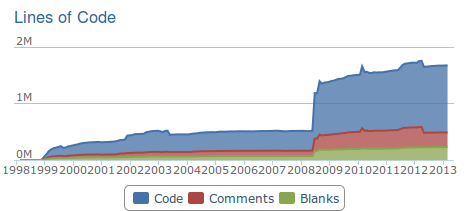
\includegraphics[width=0.7\textwidth]{thunderbird-code-evolution.png}
\caption{Thunderbird code evolution}
\label{}
\end{figure}

Thunderbird lines of code evolution jumps in 2009, filled with test classes

\subsection{How to Contribute}

There are many ways to contribute to Thunderbird, be a user is the first step to dive into the community:

\begin{itemize}
	\item \textit{Development} - Reporting bugs, patches and contributing with code.
	\item \textit{Q\&A} - After failling Mozilla\href{https://quality.mozilla.org/2013/03/mozilla-org-test-day/}{Friday test day}process into Thunderbird community, they changed the question to: \textit{"Do you want to contribute with test ?"} Thus they manage people and explain what and how they 'have to' test. Its an easier way to start to collaborate instead of \textit{"Someone wants to test ? go to url, test and report bugs"}. Better and easy as human way.
	\item \textit{Support} - Translations and localizations.
	\item \textit{Marketing} - Mozilla products Evangelist. Spreading the goods and benefits of MOFO products.
	\item \textit{Superheroes} - Thunderbird Contributors \href{https://support.mozillamessaging.com/es/kb/buscamos-superhroes}{starting page}inmozillamessaging.
	\item \textit{Forum} - Thunderbird \href{https://getsatisfaction.com/mozilla_messaging/}{forum} to search and generate information.
\end{itemize}
% section thunderbird-qa (end)
\section{Canonical}
\label{sec:canonical}

\par Canonical is the company that launched Ubuntu project in 2004. Founded by South African \href{http://www.markshuttleworth.com/}{Mark Shuttleworth} after a profit of 500\$ million from the sale of his  security company. \href{http://www.markshuttleworth.com/archives/4}{Decided to invest} the money to create a Linux distribution more friendly and easy to install

\begin{quote}
    \textit{"Linux for human beings"}
\end{quote}

\par So, he got in touch with \href{http://www.debian.org/index.html}{Debian} developers (which is one of the most reliable Linux distributions) to offer financial support to create a more human Linux \textit{Ubuntu}.

\par After a  controversial year because of this distribution is owned by one person, decided to create a Foundation in 2005: Ubuntu Foundation to prevent Ubuntu depended on a person or organization and was now to be directed by people. That gave decision making to community and Copyright Holder of Ubuntu to the Foundation to avoid possible distribution privatizations by a Company or a person.

\subsection{Technologies}

\par Canonical is not a software solution is a company that develops FLOSS project Ubuntu and other solutions that are not FLOSS.

\par We can take a look to Technologies used to develop Ubuntu with the community. Explained in their \href{https://wiki.ubuntu.com/}{Wiki} we summarize main goals in Get involved section and focusing our summary in Kernel development Team:

\begin{itemize}
	\item \textit{Communications}
    \begin{itemize}
	    \item \textit{Blogs} - Here is a planet that unifies all development team personal /technical blogs in one feed releated to huma project members in http://voices.canonical.com/kernelteam/.
	    \item \textit{IRC} channel \#ubuntu-kernel to get in touch with users and developers. Weekly IRC  public meeting in \#ubuntu-meeting to strengthen collaboration within the project.
	    \item \textit{Mailing List} - Mailing lists are highly used in Ubuntu, you can subscribe to contribute \href{https://lists.ubuntu.com/mailman/listinfo/kernel-team}{here}.
	    \item We run our mailing list much like the Linux Kernel Mailing List (LKML). Users can propose patches, ask questions and find general info. This list has medium traffic volume. For more info you can read https://wiki.ubuntu.com/KernelTeam/KernelPatches
    \end{itemize}
	\item \textit{Launchpad Teams} - ALM Tools from Ubuntu to deploy projects, I/BTS (Issue/Bugs Tracking System) and public roadmap.
\begin{itemize}
	\item \href{https://launchpad.net/~ubuntu-kernel-team}{Ubuntu Kernel Team} this is the moderated public team in which we interact with the Ubuntu Community.
	\item \href{https://launchpad.net/~canonical-kernel-team}{Canonical Kernel Team} this is a private team used by the Canonical Kernel Team for Canonical paid hardware enablement and other Canonical business.
\end{itemize}
	\item \textit{Contacts} - This section is special because translates developers to humans to get in touch with them, is based on the philosophy.
\end{itemize}

\subsection{How to Contribute}

\par \href{https://wiki.ubuntu.com/UbuntuDevelopment}{Ubuntu Development} describes a guide of how to contribute, collaborate and communicate in team projects. Ubuntu describes a community \href{http://www.ubuntu.com/project/about-ubuntu/conduct}{Code of Conduct}. A must read document that explains relations inside Ubuntu community, respect, responsible, collaborate, teamwork, meritocracy, ask for help. All rules to guide a respectful community teamwork based in communication and consensus. You \textbf{have to sign this contract} to contribute to Ubuntu community.

\par Encourages you to subscribe to mailing lists and start reading information about the community and how work internally.

\par After that take a look to bug section managed by \href{https://wiki.ubuntu.com/BugSquad}{BugSquads}. Here you can contribute searching and reporting bugs by your own or join a bug team specialized in a module. Bug Squad has a guide of their job described to triaging:

\begin{itemize}
	\item Responding to new bugs as they are filed.
	\item Ensuring that new bugs have all the necessary information.
	\item Assigning bugs to the proper package.
	\item Confirming bug reports by trying to reproduce them.
	\item Setting the importance of bugs reports. (Bug Control members Only)
	\item Searching for and marking duplicates in the bug tracking system.
	\item Sending bugs to their upstream authors, when applicable.
	\item Cross-referencing bugs from other distributions.
	\item Expiring old bugs.
\end{itemize} This section is very interesting because they are like bug soldiers inside a QA \textit{users} team and have a clear and strict workflow to deal with bugs.

\par \href{http://uds.ubuntu.com/}{Ubuntu Developer Summit} is an open-innovation section:

\begin{quote}
    \par \textit{"The bulk of UDS is discussion sessions. We explore problems and develop solutions together, pooling our collective experience"}
\end{quote}

\par Includes developers, proposals, technical users through the common idea to unify roads and problems, to create a team, nearly through the exchange of ideas and views. A good proposal for collaboration in the community.

% section canonical (end)
\section{OSOR}
\label{sec:osor}

\par \href{https://joinup.ec.europa.eu/page/osor.eu}{Open Source Observatory Repository} - Free Libre Open Source Software \textit{- FLOSS -} Forge oriented to European Public Administration. Giving a technic base and guidelines to develop FLOSS projects throught good practices. Projects has to be licensed with \href{http://joinup.ec.europa.eu/software/page/eupl/licence-eupl}{EUPL} European Union Public License. \textit{Only} Public Administrations funded FLOSS project can be hosted in OSOR you can not advertise a project by yourself.

\par The project started in 2007 and in December 2011 migrated to \href{https://joinup.ec.europa.eu/page/osor.eu}{JoinUP} the new development platform.

\subsection{Development Tools}

\par OSOR main goal is to create Communities for each FLOSS project thus create an environment in a common place to all Public Administration developments.

\begin{itemize}
	\item \textit{\href{http://gforge.com/gf/}{Gforge}} - Base for the FLOSS Forge that became Fusion Forge in 2009 (http://blog.bitergia.com/2012/11/16/the-history-of-fusionforge-and-gforge/). Strong communication with Gforge community.
	\item \textit{Repository} - Apache \href{http://subversion.apache.org/}{Subversion} for source code management.
	\item \textit{CMS -} Service for users \href{http://plone.org/}{Plone CMS}
	\item \textit{Mailing list} - \href{http://www.gnu.org/software/mailman/}{GNU Mailman}.
\end{itemize}\textit{I couldn't found more information about development tools for the project.}

\subsection{How to contribute}

\par The project ended in December 2011 so is not possible to collaborate in this project, there is no community supporting the project. Is a FLOSS project thus everyone could continue its development or play with the code to learn.

\par This summarizes community management ROLES big picture inside OSOR project A.K.A. \textit{Cheerleaders}:

\begin{itemize}
	\item \textbf{Cheerleadears} - People dedicated to spread OSOR and advertise the goodnesses of using OSOR.
\begin{itemize}
	\item \textit{News} - \href{https://twitter.com/Sjig}{Gijs Hillenius} - Journalist specialized in FLOSS and communication with other FLOSS communities, promoting workshops, events and meetings between communities.
	\item \textit{Coordination} - \href{http://www.unisys.com/unisys/}{Unisys} Ismael Olea (\href{https://twitter.com/olea}{@olea}) spreading OSOR use in Europe.
	\item \textit{Dynamizer} - \href{http://www.gopa-cartermill.com/}{GOPA}
\end{itemize}
\end{itemize}

% section osor (end)
\section{KDE}
\label{sec:kde}

\par KDE is a Desktop ? an environment ? What is KDE ? KDE started being a Desktop environment. Was founded in 1996 by Matthias Ettrich looking for the creation of a working and intuitive Desktop Environment for Unix distributions with common applications to create an ecosystem.

\par The projects evolved using Qt framework which became FLOSS software in 1998 and the first version KDE 1.0.

\par Continued evolving and growing with user until this transformation in 2009 into a FLOSS developers community, not only Desktop environment. Thus KDE wanted to spread the use of Free Software in desktops, without focusing on the development of the desktop environment. The foundation covers most fields of product development for desktop. Thus trying to spread the use of Free Software in all levels of users. It is an ambitious but successful.

\subsection{Technologies}

\par Development in KDE is divided in different sections:

\begin{itemize}
	\item \textit{Core Tools} - CMake and VCS tool, Git or SVN. Basic tools to build.
	\item \textit{Debugging and Analysis} - Tools for debugging KDE projects are composed by Valgrind, The GNU Project Debugger (GDB), KDbg and DDD, MS Windows tools.
	\item \textit{Development Tools} - A set of IDEs to develop KDE projects: Qt Creator, KDevelop, MS Visual Studio® Express IDE (Windows only)
	\item \textit{Internationalization (i18n) Tools} - Set of internationalization tools to contribute easily - Lokalize, Dr. Klash, The x-test language.
\begin{itemize}
	\item \textit{Examining .po files}
\end{itemize}
	\item \textit{Helper Tools} - Get information about KDE's installation - kde-config, Driving Konqueror From Scripts - kfmclient, Updating User Configuration Files - kconf\_update, Generating apidox, Automoc4, svnmerge.py
	\item \textit{Quality Assurance} - Code Review, Continuous Building, English Breakfast Network - Static Analysis
\end{itemize} Detailed information can be found in \href{http://techbase.kde.org/Development/Tools}{http://techbase.kde.org/Development/Tools}. TechBase KDE is a place made to share knowledgement for everyone. Was created after KDE became more than a Desktop Client (first edition of Development Tools in 2006).

\subsection{How to contribute}

\par How to become a committer ? You can ask any community member for this permission. It's a community with easy entry and likes to receive new members.

\par After this point, you have to work on it following community guidelines. The steps aren't different from other communities, we can see a common pattern in communities:

\begin{itemize}
	\item \textit{News and Mail Sources} - Mailing lists, history and news.
	\item \textit{Reporting Bugs} - Bug reporting and bug fixing.
	\item \textit{Getting Started with Coding}:  C++, Qt,  KDE - Yes, you have to code to contribute to development.
	\item \textit{Getting Involved in Bug Hunting and Application Quality} - Be a Quality Assurance expert helping improving test and quality. 
	\item \href{http://community.kde.org/KDE/Junior_Jobs}{\textit{Junior Bugs}} - This is a special part to get in touch with the community, an easy way to start fixing bugs and know how to work in community.
	\item \textit{User Interface} - Avoid flames about UI \textit{"User interface is a very wide subject".}
	\item \textit{Getting Answers to Your Questions} - Learn to search and use documentation. It's very important to read the FAQs, mail lists, documentation, wikis, bugs before post anything because could be duplicated and become a nonsense effort
\end{itemize}

\par Extended guide could be found at \href{http://techbase.kde.org/Contribute}{http://techbase.kde.org/Contribute}.

% section kde (end)

\section{Differences and Similarities}
\label{sec:differences-and-similarities}

\par Using matrix visualization we are going to appreciate differences and similarities between contributions access guidelines through project communities analyzed in talks checking:

\begin{itemize}
	\item \emph{Mailing lists} -  Mailing list such as developers, users, etc\ldots
	\item \emph{Developer Guide} - Documentation for start development environment.
	\item \emph{Bug Tracking System} - Bug or Issue tracking system to manage project resources and schedules.
	\item \emph{Mentoring program} - Mentoring program to introduce new users to produce upstream in the community and guide them into the process with another members of the community.
	\item \emph{Forum} - Forum, FAQs or other tool to interact the community creating community.
	\item \emph{Documentation} - Project documentation for every type of user, from technical to end-user (if exists).
\end{itemize}

\begin{center}
    \textbf{Y} - \emph{Yes}, \textbf{N} - \emph{No}, \textbf{N/A} - \emph{Not Available}
\end{center}

\begin{center}
    \begin{tabular}{ | l | c | c | c | c | c | c | }
        \hline
        & \textbf{Mail list} & \textbf{Dev Guide} & \textbf{BTS} & \textbf{Mentoring} & \textbf{Forum} & \textbf{Documentation} \\ \hline
        \hline 
        \emph{Apache}              & Y & Y & Y & Y & \textbf{N} & Y \\ \hline
        \emph{WebKit}              & Y & Y & Y & \textbf{N} & \textbf{N} & Y  \\ \hline
        \emph{Plan9}               & Y & Y & \textbf{N} & \textbf{N} & \textbf{N} & Y \\ \hline
        \emph{Mozilla}             & Y & \textbf{N} & Y & \textbf{N} & Y & Y  \\ \hline
        \emph{GNU}                 & Y & Y & Y & \textbf{N} & \textbf{N} & Y \\ \hline
        \emph{Open Document}       & Y & Y & Y & Y & Y & Y \\ \hline
        \emph{Libre Desktop}       & \textbf{N/A} & \textbf{N/A} & \textbf{N/A} & \textbf{N/A} & \textbf{N/A} & \textbf{N/A} \\ \hline
        \emph{Wikipedia}           & Y & Y & Y & Y & Y & Y \\ \hline
        \emph{Liferay}             & Y & Y & Y & \textbf{N} & Y & Y \\ \hline
        \emph{AZLinux Migration}   & \textbf{N/A} & \textbf{N/A} & \textbf{N/A} & \textbf{N/A} & \textbf{N/A} & \textbf{N/A} \\ \hline
        \emph{GNOME}               & Y & Y & Y & \textbf{N} & \textbf{N} & Y \\ \hline
        \emph{Thunderbird}         & Y & Y & Y & \textbf{N} & Y & Y\\ \hline
        \emph{Canonical/Ubuntu}           & Y & Y & Y & \textbf{N} & Y & Y \\ \hline
        \emph{OSOR}                & \textbf{N/A} & \textbf{N/A} & \textbf{N/A} & \textbf{N/A} & \textbf{N/A} & \textbf{N/A} \\ \hline
        \emph{KDE}                 & Y & Y & Y & Y & Y & Y \\ \hline
    \end{tabular}
\end{center}

% section differences-and-similarities (end)

\section{Conclusions}
\label{sec:conclusions}

\par Taking a first look into the result table we can remove data that can't be evaluated from projects such as:
\begin{itemize}
	\item \emph{Libre Desktop} - The talk was related to how the law evolved to IT and FLOSS during last 30 years in Spain.
	\item \emph{AZLinux Migration} - Migration to FLOSS in Public Administrations. This project as is explained is more important to spread this results that contribute because is a process not a FLOSS project by itself.
	\item \emph{OSOR} - OSOR Project disappear in December 2011 so, development and contributions doesn't already exist for our misfortune.
\end{itemize}

\par The following leads out to \emph{Mentoring} column. There are a lot of projects (analyzed in the talks) that do not involve mentoring 5 to 7. Those projects that use some kind of mentoring (interactive manuals guided by a another user/s) are more focused to end-user (non technical) that others. Their marketing is related to more 'tangible' projects for the 'real world' like Wikipedia, KDE, Open Document and Apache ? I think they have more 'human' part than the others and because of that they produce these mentoring programs.

\par Other remarkable point are the \emph{Forums}. Surprised when I saw the results that projects like GNOME doesn't have official forums, neither than WebKit a project used worldwide and covers many fields. These projects work with what they need, it is always better \textbf{to know that you do not need}.

\emph{Jono Bacon} in Art-of-community introduction to \emph{Communicating Clearly} chapter:
\begin{quotation}
    \emph{"Community is absolutely about understanding the ether. Our notes are the processes, governance, tools, and methods in which we work together. The notes we don’t play are the subtle nuances in how we pull these notes together and share them with one another. The space between the notes is communication."}
\end{quotation}

\par In the opposite hand we have Open Document community that works great with them forums as Charles told us.

\par In closing, I wish to emphasize a conclusion on the final paragraph. The communities studied have their little rules to run through his life. As people also find it difficult to change because all change is associated with ignorance and uncertainty. What I mean is that each one works in a way through standards but underneath all, absolutely all, are communities of people who rely on the cooperation and communication between them.

\par We can not draw generic standards for the communities studied with the data we have exposed. It's a small study on a roughly speeches in the course classes 'Case Studies II' and the amount of research work on FLOSS communities.

% section conclusions (end)
\end{document}